% !TeX root = ..\rapport_13_1.tex
\section{Kravspecifikation}
\subsection{Indledning}
\subsection{Ordliste}
\begin{table}[H]
    \centering
    \caption{Liste over gloser brugt i dette projekt og disses beskrivelser.}\label{tbl:gloser}
    \begin{tblr}{width = \textwidth, colspec={Q[l, font = \bfseries, wd = .2\textwidth]Q[l, wd = .7\textwidth]}}
        \toprule
        Aktivitet         & En opgave med tilknyttet varighed, medarbejdere kan deltage i at udføre.                                            \\
        Faste aktiviteter & Aktiviteter der ikke kan pålægges et projekt. F.eks. ferie, sygdom, kurser.                                         \\
        Projekt aktivitet &                                                                                                                     \\
        Projekt           & Samling af aktiviteter, enten internt (dvs. at projektet er Softwarehuset A/S' eget) eller eksternt (for en kunde). \\
        Medarbejder       & Alias udviklingsmedarbejder; de som står for udviklingen af softwareløsninger til kunder.                           \\
        Kunde             &                                                                                                                     \\
        Projektleder      & En medarbejder valgt blandt udviklingsmedarbejdere                                                                  \\
        Softwarehuset A/S & Kunden til softwareløsningen                                                                                        \\
        Medarbejder ID    & Initialer på 4 bogstaver. F.eks. huba                                                                               \\
        Projektnumre      & Har formen årstal og et løbenummer. F.eks. 22001                                                                    \\
        Varighed          & En aktivitets fastlagte antal timer                                                                                 \\
        Arbejdstid        & Mængde tid i inkrementer af halve timer, brugt på en aktivitet                                                      \\
        \bottomrule
    \end{tblr}
\end{table}
\subsection{Use case diagrams}
\subsubsection{Projektstyring}

\begin{figure}[H]
    \centering
    \caption{Use case: Projektstyring}\label{fig:Projektstyring}
    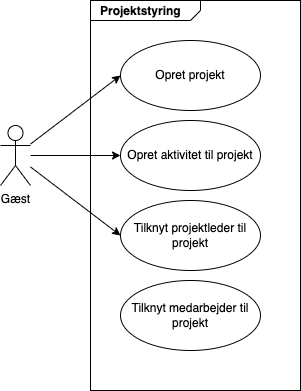
\includegraphics[width=.3\textwidth]{Diagrams/guest_project}
\end{figure}

\subsubsection{Aktivitetshåndtering}

\begin{figure}[H]
    \centering
    \caption{Use case: Aktivitetshåndtering}\label{fig:Aktivitetshaandtering}
    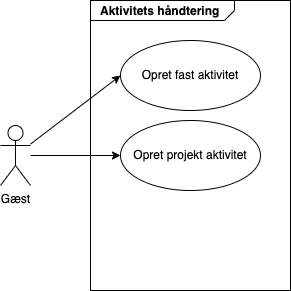
\includegraphics[width=.3\textwidth]{Diagrams/guest_activity}
\end{figure}

\subsubsection{Bruger administration}

\begin{figure}[H]
    \centering
    \caption{Use case: Bruger administration}\label{fig:BrugerAdmin}
    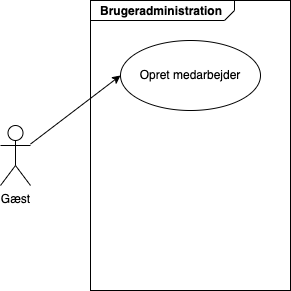
\includegraphics[width=.3\textwidth]{Diagrams/guest_users}
\end{figure}

\subsection{Detaljerede use cases}
\subsection{Opret projekt}
\Large{Kaspers udkast af use case}\newline
\normalsize
\emph{Navn}\newline
Opret projekt\newline
\emph{Beskrivelse}\newline
Der kan oprettes projekter\newline
\emph{Aktør}\newline
Bruger
\begin{figure}[H]
    \centering
    \caption{Det her var et forsøg på at lave et use-case diagram med alle actors tilstede. Der er muligvis også flere use-cases end nødvendig, men de her er stillet af opgaven, som fremgår af projektbeskrivelsen. Ikke nødvendigvis det mest overskuelige use-case diagram, men en fordel ved denne er - selvom det er en mindre detalje - at man får en enkel use-case relation med, nemlig <<extend>>. (Mathies)}\label{fig:AlleActorsPaaEnGang}
    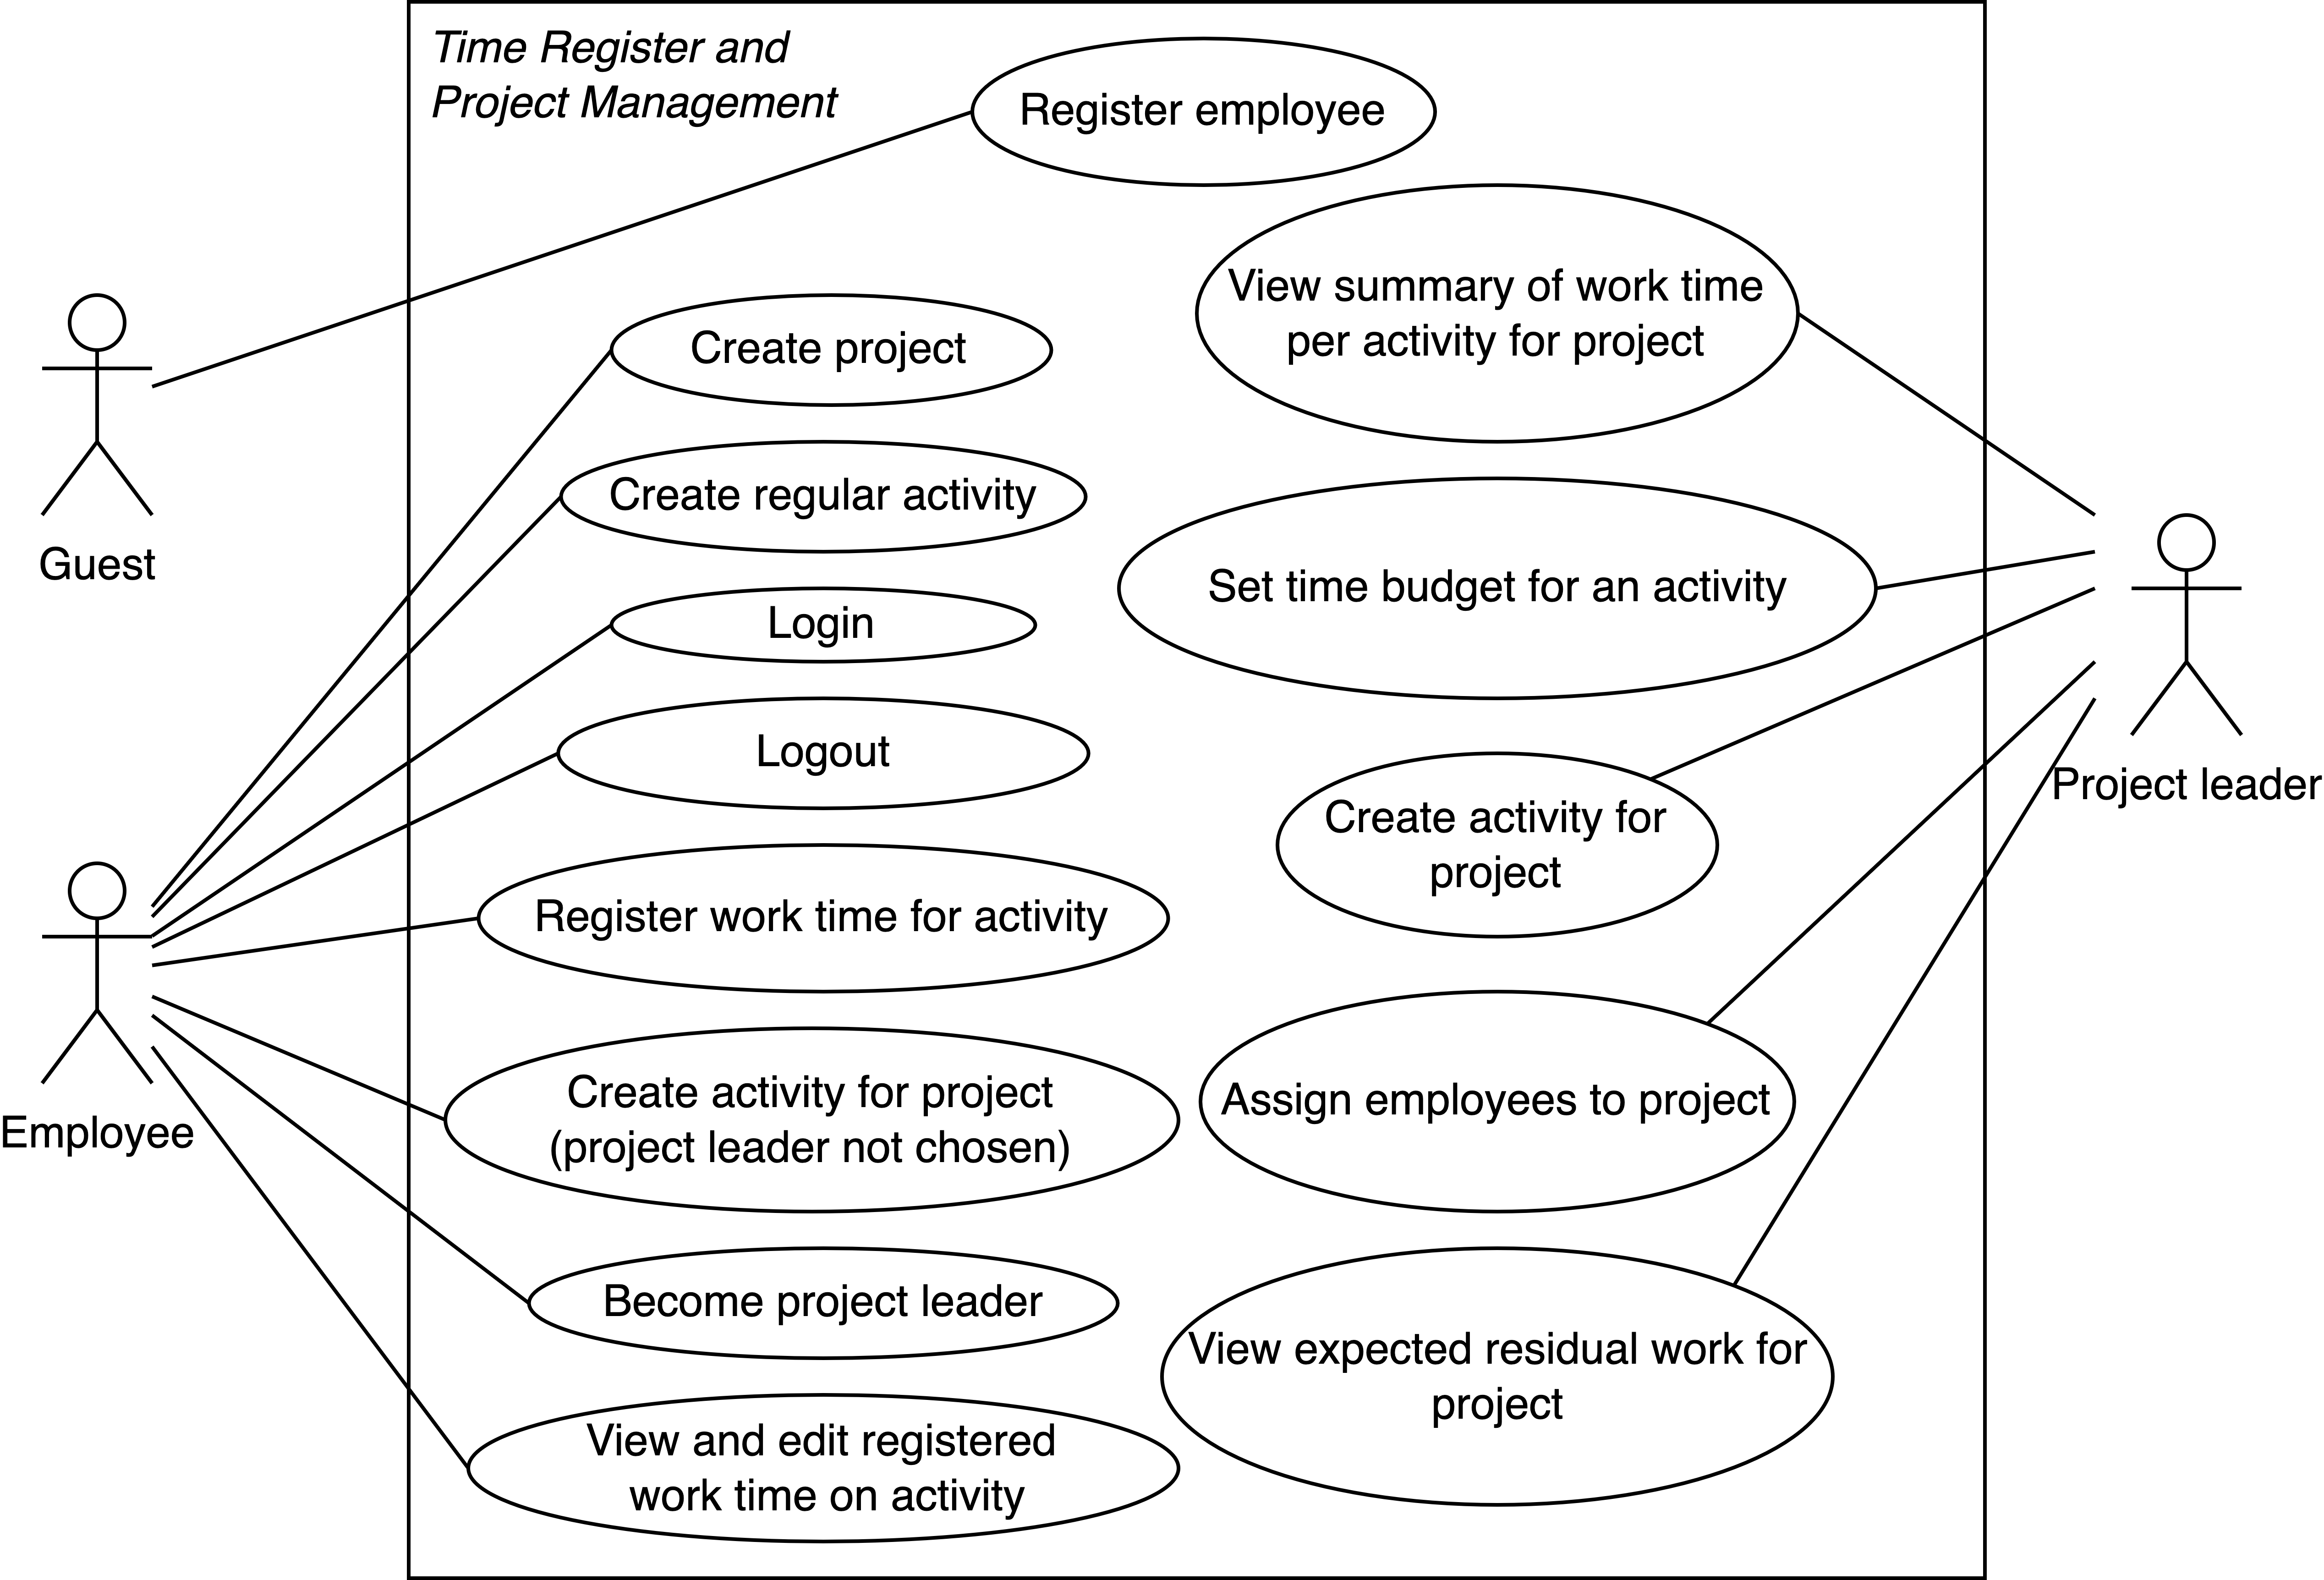
\includegraphics[width=.7\textwidth]{Diagrams/Timeregistrering og projektstyring.png}
\end{figure}

% \emph{Cucumber feature 1}
% \begin{verbatim}
% Feature: Buy fruit
% Description: A user buys fruit...
% Actors: User

% Scenario: Buy a fruit with enough money
%     Given the vending machine has fruits
%     When the user enters enough mone for a fruit
%     And the user selects a fruit
%     And the machine returns the rest money
%     And the vending machine remembers its earnings
%     ...
    
% \end{verbatim}
\begin{listing}[H]
    \centering
    \caption{Cucumber feature 1}\label{lst:feature1}
    \begin{minted}{gherkin}
    Feature: Buy fruit
    Description: A user buys fruit...
    Actors: User
    
    Scenario: Buy a fruit with enough money
        Given the vending machine has fruits
        When the user enters enough mone for a fruit
        And the user selects a fruit
        And the machine returns the rest money
        And the vending machine remembers its earnings
        ...
    \end{minted}
\end{listing}